Air pollution is the leading environmental health risk in many areas around the world.
The effects of air pollution to the general population range from chronic to less severe health impacts and reduced growth rates of vegetation resulting in economic losses of billions of euros \citep{AQEU:2015}.
Moreover, the International Agency for Research on Cancer labelled air pollution as carcinogenic \citep{IARC:2013}.
Due to these impacts, many governed areas introduced legislation designed to reduce concentrations of many air pollutants.

Tropospheric ozone (\ce{O3}) is one of the most problematic air pollutants over Europe with up to $98$~\% of Europe's urban population exposed to concentrations of ozone above the WHO guidelines \citep{AQEU:2015}.
Furthermore, in 2011 the EU ozone target value for human health (the EU has no limit value for ozone) was exceeded in $65$~\% of the EU member states and Europe's ozone target value for vegetation was exceeded in $27$~\% of the EU-28 agricultural areas \citep{AQEU:2013}.

Reducing atmospheric concentrations of tropospheric ozone is a complex problem as ozone is not directly emitted into the troposphere.
Tropospheric ozone is produced from the reactions of volatile organic compounds (VOCs) in the presence of nitrogen oxides \mbox{(\ce{NO_x}~$\equiv$~NO + \ce{NO2})} and sunlight \citep{Atkinson:2000}.
Meteorology and transport also influence tropospheric ozone levels \citep{Jacob:2009}.

Air quality (AQ) models are an important tool for understanding ozone pollution and predicting future air quality.
Many AQ models are available with different scales and dimensions depending on the scope of the modelling experiment.
Accurately representing the complexity of ozone production in a computationally efficient model is an ongoing challenge for the modelling community \citep{Russell:2000}.

Model intercomparison projects (MIPs) compare the outputs from different models showing differences in tropospheric ozone due to differing representations of key processes.
For example, ACCMIP (Atmospheric Chemistry and Climate Model Intercomparison Project) showed different magnitudes of future ozone burden in the same region \citep{Young:2013}.
A current MIP, CCMI (Chemistry Climate Model Initiative), aims to investigate differences in the representation of chemistry, emissions and transport processes between models to understand the differences between predictions from global models \citep{Eyring:2013}.

Detailed process studies are key to understanding differences between simulated ozone levels using different models.
This thesis focuses on the influence on ozone production from the representation of VOC degradation chemistry, VOC emissions and the ozone-temperature relationship within models with the research questions framing this work found in Sect.~\ref{s:research_questions}.
This assessment should be beneficial to the modelling community in understanding potential differences between model outputs and improving AQ models.
The remainder of this introduction discusses ozone in the atmosphere, the chemistry and sources of ozone as well as the effects of meteorology on ozone production.

\section{Ozone} \label{s:ozone}
%atmospheric O3 with budget, lifetime, stratospheric & tropospheric ozone
Ozone is a atmospheric gas found in the stratosphere and troposphere, however its atmospheric effects are very different in these regions.
The stratosphere contains $\sim$~90~\% of the atmospheric ozone with a peak mixing ratio of $\sim$~$12$~ppm \citep{Seinfeld:2006}.
Stratospheric ozone absorbs the sun's ultraviolet radiation which is important due to the adverse effects of excess UV radiation on humans and ecosystems.

In contrast, tropospheric (or surface) ozone is both a pollutant and a greenhouse gas. 
Increased levels of tropospheric ozone are harmful to humans, plants and other living systems. 
High ozone exposure may lead to pulmonary problems in humans and can decrease both crop yields and forest growth \citep{WMO:2010}. 

Tropospheric ozone is formed via photochemical production from the reactions between VOCs and \ce{NO_x}, described in Sect.~\ref{s:ozone_chemistry}, while meteorology and atmospheric transport also influence ozone concentrations.
For example, a spring-time peak in tropospheric ozone is common in the Northern Hemisphere (NH) mid-latitudes, originally attributed to transport of ozone from the stratosphere into the troposphere via the Stratosphere-Troposphere Exchange (STE) \citep{Monks:2000}.
However, ozone transported via STE rarely influences surface ozone levels \citep{Lelieveld:2000} and the spring maximum is due to the photochemical reactions occuring in the NH spring after the buildup of reservoir species over winter \citep{Penkett:1986}.
For the rest of this thesis, ozone refers to tropospheric ozone.

Understanding the intracacies of surface ozone pollution requires a combined effort from the modelling, observational and chemical kinetic communities -- called the ``three-legged stool'' approach by \citet{Abbatt:2014}.
Modelling of ozone production helped understand the complexity of atmospheric chemistry, such as the non-linear relationship of ozone production with precursor (VOC and \ce{NO_x}) emissions.
Modelling studies attempt to reproduce observational trends of surface ozone and model predictions may inform new observational studies.
Chemical kinetic studies performed by laboratories give insights to missing or incorrect representations of atmospheric chemistry to be included in updated models.

\section{Ozone Chemistry} \label{s:ozone_chemistry}
Ozone absorbs UV radiation producing either ground-state atomic oxygen (\ce{O(^3P)}) or excited singlet (\ce{O(^1D)}) oxygen atoms.
\begin{rxnarray}
    \ce{O3 + h\nu} & \rightarrow \ce{O2 + O(^3P)} \label{r:O3_hva} \\
    \ce{O3 + h\nu} & \rightarrow \ce{O2 + O(^1D)} \label{r:O3_hvb} 
\end{rxnarray}
Ground-state oxygen quickly reacts with oxygen to reform ozone.
\begin{rxnarray}
    \ce{O(^3P) + O2} & \xrightarrow[]{\text{\tiny{M}}} \ce{O3} \label{r:O_O2}
\end{rxnarray}
Thus there is no net loss or production of ozone through \eqref{r:O3_hva} and \eqref{r:O_O2}.
\ce{O(^1D)} may collide with \ce{N2} or \ce{O2} (represented as M in chemical reactions) stabilising to the ground-state.
%\begin{rxnarray}
    %\ce{O(^1D)} & \xrightarrow[]{\text{\tiny{M}}} \ce{O(^3P)} \label{r:O1D_M} 
%\end{rxnarray}
This process again leads to a null cycle with ozone destruction balanced by production.
However, \ce{O(^1D)} can react with water vapour producing hydroxyl (OH) radicals.
The OH radical is a highly reactive chemical species reacting with almost all trace chemical species in the troposphere.
\citep{Seinfeld:2006, Monks:2005}
\begin{rxnarray}
    \ce{O(^1D) + H2O} & \rightarrow \ce{2 OH} \label{r:O1D_H2O}
\end{rxnarray} 

The initial oxidation of VOCs by OH initiates a reaction chain which may lead to net production or loss of ozone depending on the atmospheric conditions.
For example, when carbon monoxide (CO) reacts with OH in the presence of oxygen, carbon dioxide and the hydroperoxy (\ce{HO2}) radical are formed.
In polluted areas with high-\ce{NO_x} concentrations, \ce{HO2} readily reacts with nitrogen oxide (NO) regenerating OH and producing nitrogen dioxide (\ce{NO2}).
\begin{rxnarray}
    \ce{CO + OH} & \xrightarrow[]{\ce{O2}} \ce{HO2 + CO2} \label{r:CO_OH} \\
    \ce{HO2 + NO} & \rightarrow \ce{OH + NO2} \label{r:HO2_NO}
\end{rxnarray}
Photolysis of \ce{NO2} produces ground-state atomic oxygen leading to ozone production via \eqref{r:O_O2}.  
\begin{rxnarray}
    \ce{NO2 + h\nu} & \rightarrow \ce{NO + O(^3P)} \label{r:NO2_hv} 
\end{rxnarray}
%OH may also react with NO to produce nitrous oxide (HONO), which rapidly photolyses to return OH and NO.
%\begin{rxnarray}
    %\ce{OH + NO} & \rightarrow \ce{HONO} \label{r:OH_NO} \\
    %\ce{HONO + h\nu} & \rightarrow \ce{OH + NO} \label{r:HONO_hv}
%\end{rxnarray}
The reaction between OH and \ce{NO2} produces nitric acid (\ce{HNO3}) limiting the recycling of OH and \ce{NO2}.
Nitric acid may be removed through deposition and is a sink for both OH and \ce{NO2}.
\begin{rxnarray}
    \ce{NO2 + OH} \rightarrow \ce{HNO3} \label{r:NO2_OH}
\end{rxnarray}

In low-\ce{NO_x} conditions away from polluted areas, OH and \ce{HO2} are interconverted through reactions with ozone.
\begin{rxnarray}
    \ce{OH + O3} & \rightarrow \ce{HO2 + O2} \label{r:OH_O3} \\
    \ce{HO2 + O3} & \rightarrow \ce{OH + 2 O2} \label{r:HO2_O3}
\end{rxnarray}
OH and \ce{HO2} may also react in a termination reaction producing water vapour and oxygen.
\begin{rxnarray}
    \ce{HO2 + OH} \rightarrow \ce{H2O + O2} \label{r:HO2_OH}
\end{rxnarray}
Other termination reactions involve combination reactions of \ce{HO2} radicals producing hydrogen peroxide (\ce{H2O2}).
\begin{rxnarray}
    \ce{HO2 + HO2} & \rightarrow \ce{H2O2} \label{r:HO2_HO2}
\end{rxnarray}
Hydrogen peroxide may be removed through deposition \citep{Gunz:1990} but may also be a temporary sink for the odd-oxygen species OH and \ce{HO2}.
\begin{rxnarray}
    \ce{H2O2 + h\nu} & \rightarrow \ce{2 OH} \label{r:H2O2_hv} \\
    \ce{H2O2 + OH} & \rightarrow \ce{HO2 + H2O} \label{r:H2O2_OH}
\end{rxnarray}
In summary, the secondary degradation of CO produces ozone in high-\ce{NO_x} conditions while in low-\ce{NO_x} conditions ozone is destroyed.
\citep{Seinfeld:2006, Monks:2005}

\begin{figure}[t]%
    \begin{center}%
        \caption[Methane degradation pathways]{Methane degradation pathways in low-\ce{NO_x} and high-\ce{NO_x} conditions. Taken from \citet{Monks:2005}.}%
        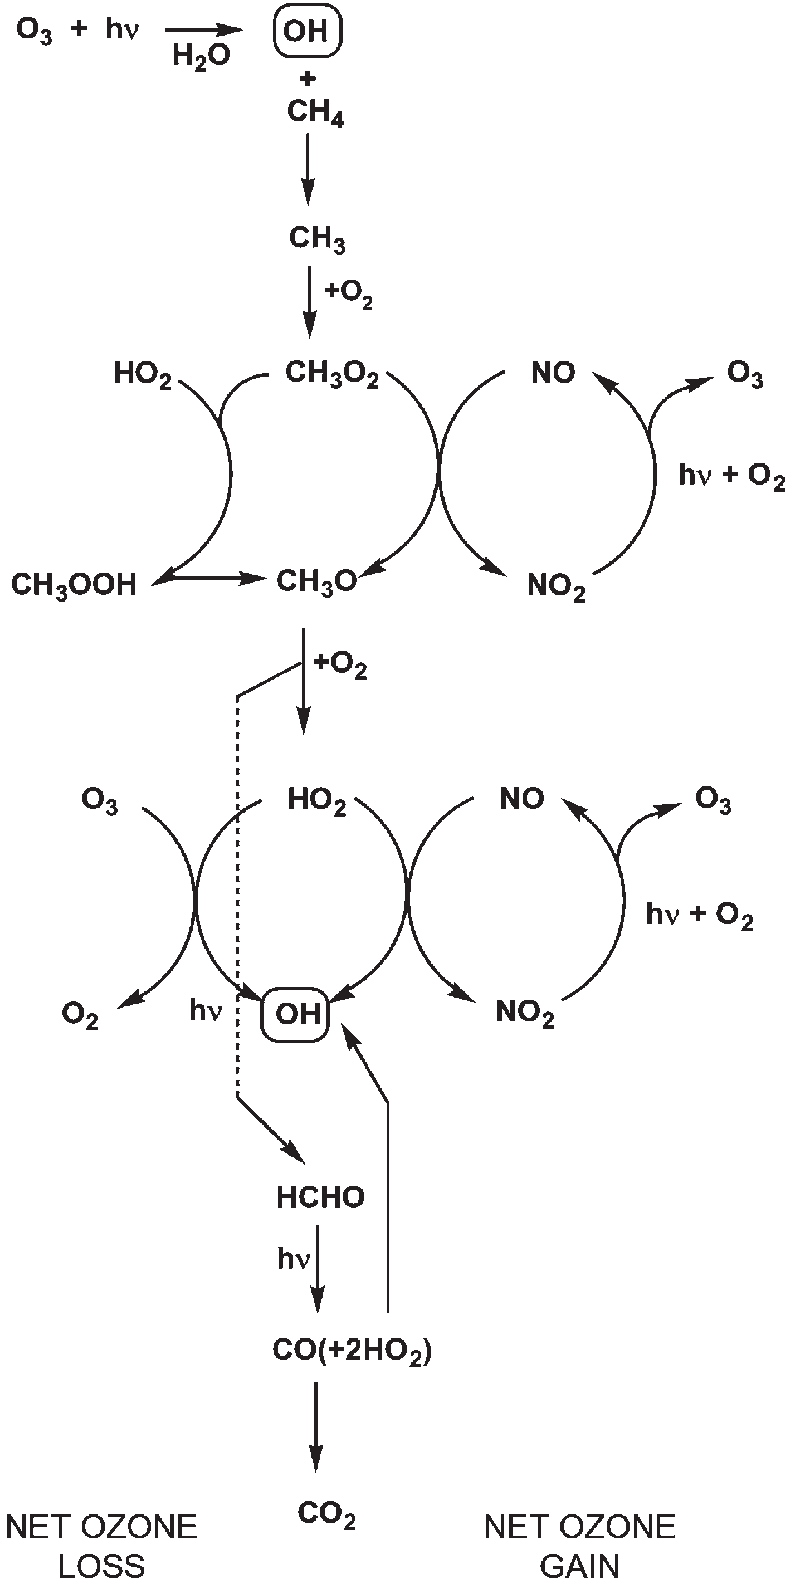
\includegraphics[scale = 0.45]{CH4_degradation}%
        \label{f:CH4_oxidation}%
    \end{center}%
\end{figure}%
The secondary degradation of more complex VOCs has similar features to that of CO.
Methane (\ce{CH4}), with a mixing ratio of $\sim$~$1.7$~ppmv, is the most abundant VOC in the troposphere.
The reaction of \ce{CH4} with OH, in the presence of \ce{O2}, produces the methyl peroxy radical (\ce{CH3O2}) -- the simplest organic peroxy radical (\ce{RO2}).
\begin{rxnarray}
    \ce{CH4 + OH} \xrightarrow[]{\ce{O2}} \ce{CH3O2 + H2O} \label{r:CH4_OH}
\end{rxnarray}
Similar to CO oxidation, \ce{NO_x} conditions play a crucial role in the fate of \ce{CH3O2} and whether ozone is produced or destroyed, depicted in Fig.~\ref{f:CH4_oxidation}.

\begin{figure}[t]%
    \begin{center}%
        \caption[Schematic of general secondary degradation of VOCs]{Schematic diagram outlining general pathways of the secondary degradation of an emitted VOC.}%
        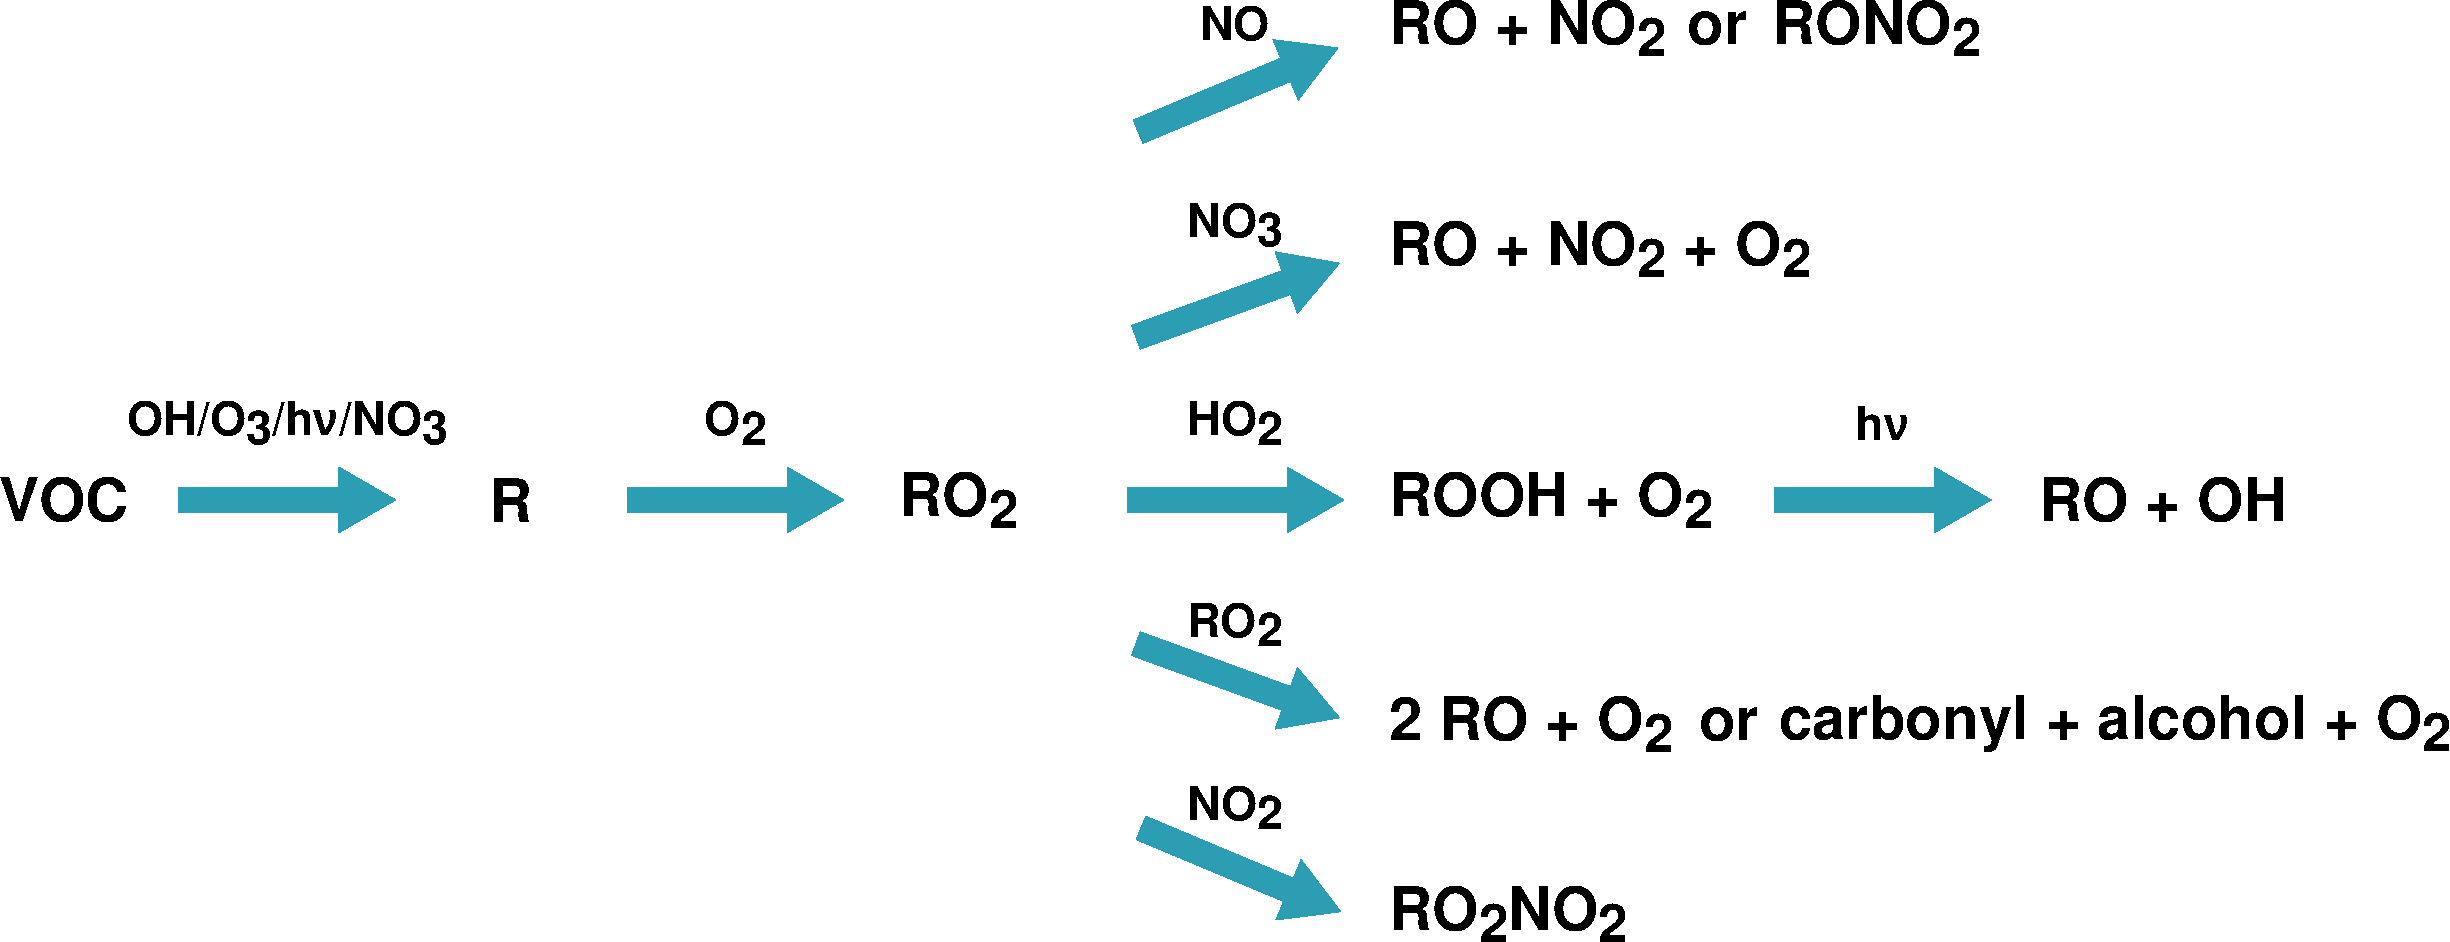
\includegraphics[width = \textwidth]{VOC_degradation}%
        \label{f:VOC_reaction}%
    \end{center}%
\end{figure}%
The general types of secondary degradation products formed during \ce{CH4} degradation can be extended to more complex non-methane VOCs (NMVOCs).
Initial oxidation pathways of NMVOCs are reaction with OH, while unsaturated VOCs, such as alkenes, may react with ozone and photolysis is important for carbonyl species.
During the night-time, reaction with the nitrate (\ce{NO3}) radical is typically more important than OH-oxidation due to the relatively higher night-time concentrations of \ce{NO3}.
\begin{rxnarray}
    \ce{VOC + OH / NO3 / O3 / h\nu} & \xrightarrow[]{\ce{O2}} \ce{RO2} \label{r:VOC_init} 
\end{rxnarray} 

Figure~\ref{f:VOC_reaction} represents a general and simplified reaction scheme for VOCs in the troposphere. 
The initial oxidation of NMVOC produces \ce{RO2} radicals and the fate of the \ce{RO2} determines whether net loss or production of ozone occurs.
\begin{rxnarray}
    \ce{RO2 + NO} & \xrightarrow[]{\text{M}} \ce{RONO2} \label{r:RO2_NOa} \\
    \ce{RO2 + NO} & \rightarrow \ce{RO + NO2} \label{r:RO2_NOb} \\
    \ce{RO2 + NO2} & \xrightleftharpoons[]{\text{M}} \ce{RO2NO2} \label{r:RO2_NO2} \\
    \ce{RO2 + NO3} & \rightarrow \ce{RO + NO2 + O2} \label{r:RO2_NO3} \\
    \ce{RO2 + HO2} & \rightarrow \ce{ROOH + O2} \label{r:RO2_HO2} \\
    \ce{RO2 + RO2} & \rightarrow \ce{2RO + O2} \label{r:RO2_RO2a} \\
    \ce{RO2 + RO2} & \rightarrow \ce{RCH(OH)R + RC(O)R + O2} \label{r:RO2_RO2b}
\end{rxnarray}
All degradation pathways of \ce{RO2} that produce \ce{NO2} result in \ce{O3} formation due to \eqref{r:NO2_hv} and \eqref{r:O_O2}. 
Reaction with \ce{HO2} forms a hydroperoxide (ROOH) which may either be deposited or photolysed producing an alkoxy (RO) radical and OH.
The carbonyl and alcohol products resulting from reactions between \ce{RO2} radicals follows a similar sequence of reactions and can produce further \ce{O3}. 
Thus the subsequent reactions of secondary degradation products of a VOC may lead to further production of ozone.

Reaction of \ce{RO2} with \ce{NO2} \eqref{r:RO2_NO2} forms peroxy nitrates (\ce{RO2NO2}) which are a temporary reservoir for \ce{RO2} and \ce{NO_x}.
The thermal decomposition rate of \ce{RO2NO2} is highly temperature dependent.
At lower temperatures, \ce{RO2NO2} builds up and may be transported away from the region of formation. 
Thus releasing \ce{RO2} and \ce{NO2} in areas away from large sources of \ce{NO_x} and fuelling ozone production.
%This is one example of the dependence of ozone production on meteorological variables, a broader overview is given in Sect.~\ref{s:meteo_ozone}.

The reaction between NO and ozone is another important reaction in polluted regions.
\begin{rxnarray}
    \ce{NO + O3} & \rightarrow \ce{NO2 + O2} \label{r:NO_O3}
\end{rxnarray}
Together with \eqref{r:NO2_hv} and \eqref{r:O_O2}, \eqref{r:NO_O3} form a null cycle of ozone production and destruction which limits ozone levels.
On the local urban scale close to NO sources, \eqref{r:NO_O3} decreases ozone levels called ozone titration.
Ozone titration is also important during the night where the lack of photochemistry does not regenerate ozone.
Urban measurement studies have confirmed the importance of ozone titration near sources of NO \citep{Syri:2001}.

\subsection[VOC and NOx Chemistry]{VOC and \ce{NO_x} Chemistry} \label{ss:VOC_NOx}
\begin{figure}[t]%
	\begin{center}%
        \caption[Ozone mixing ratios as a function of \ce{NO_x} and VOCs]{Ozone isopleth plots for various initial mixing ratios of \ce{NO_x} and VOCs. Taken from \citet{Jenkin:2000}.}%
        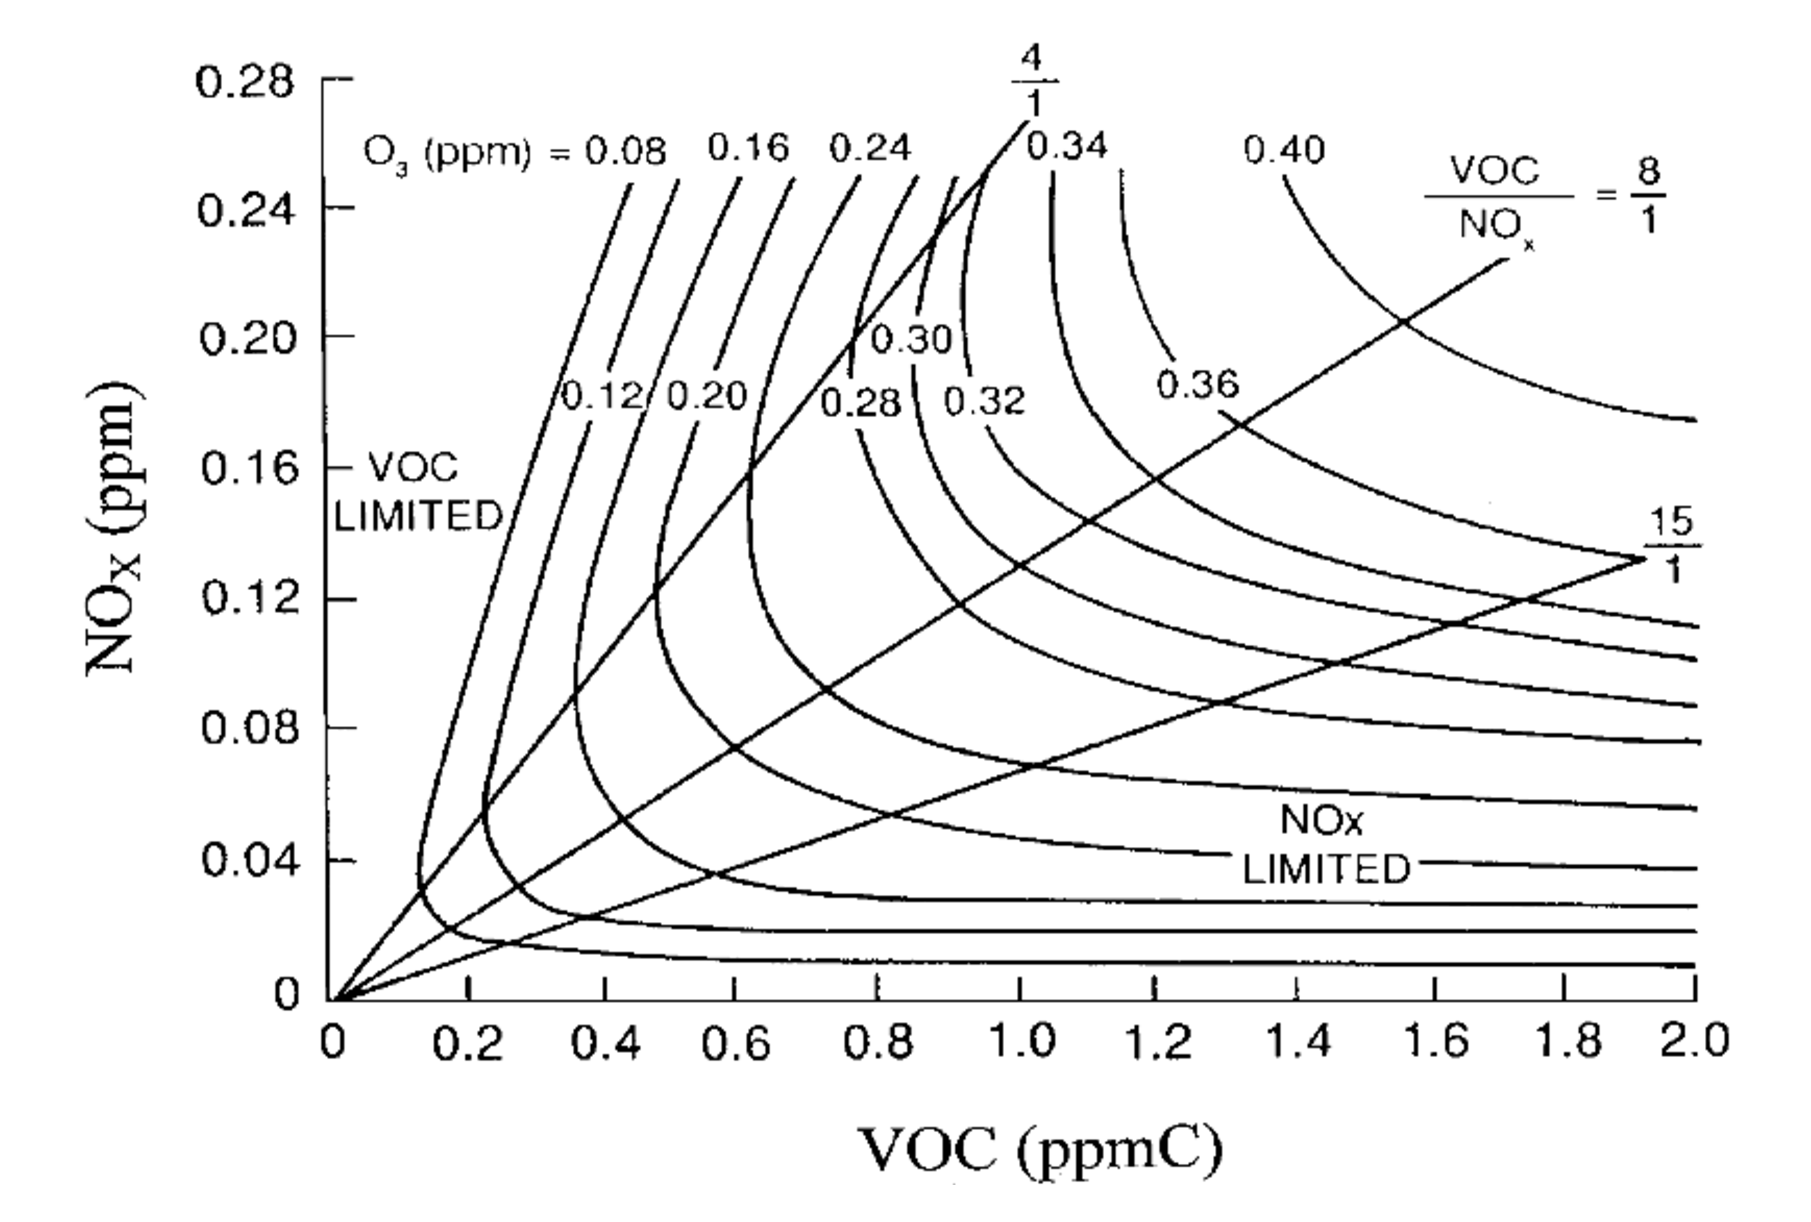
\includegraphics[width = 0.9\textwidth]{O3_isopleth}%
		\label{f:O3_isopleth}%
	\end{center}%
\end{figure}%
The chemistry in low-\ce{NO_x} and high-\ce{NO_x} conditions indicates that ozone production is a non-linear process.
Figure~\ref{f:O3_isopleth}, from \citet{Jenkin:2000}, depicts the non-linear relationship between ozone as a function of VOC and \ce{NO_x}.
This relationship can be divided into distinct regimes of ozone production: \emph{\ce{NO_x}-sensitive} (or \emph{\ce{NO_x}-limited}), \emph{\ce{NO_x}-saturated} (or \emph{VOC-limited}) and \emph{VOC-and-\ce{NO_x}-sensitive} regimes. 

%balance of NOx & NMVOC for O3 production
%The fate of peroxy radicals produced during VOC degradation depends on the ratio of the concentrations of radicals and \ce{NO_x} \citep{Kleinman:1991, Kleinman:1994}.
In regions with low-\ce{NO_x} concentrations, \ce{RO2} are more likely to react with other radicals rather than convert NO to \ce{NO2} leading to ozone production.
%The most common reactions are bimolecular destruction \eqref{r:HO2_OH}, which removes radicals, or combination of radicals \eqref{r:RO2_HO2} into reservoir species that may re-release radicals.
Increasing \ce{NO_x} levels increases the number of NO to \ce{NO2} conversions by peroxy radicals leading to ozone production.
While, increasing VOC levels has little effect on \ce{O3} production due to increased radical-radical reactions.
This is \emph{\ce{NO_x}-sensitive} chemistry.  

On the other hand in regions with high levels of \ce{NO_x}, reactions between radicals and \ce{NO_x} are more likely to occur.
The production of \ce{HNO3} increases through \eqref{r:NO2_OH} removing OH and \ce{NO2}.
Increasing levels of VOC increase the likelihood of \ce{RO2} converting NO to \ce{NO2} leading to ozone production while increasing \ce{NO_x} levels will not increase \ce{O3} production.  
This is \emph{\ce{NO_x}-saturated} or \emph{VOC-limited} chemistry.

The VOC-and-\ce{NO_x}-sensitive regime (contour ridges in Fig.~\ref{f:O3_isopleth}) is characterised by \ce{O3} production being sensitive to both VOC and \ce{NO_x} levels. 
Morever, it is in this atmospheric regime that the maximum amount of ozone is produced.
\citet{Kleinman:1994} showed that this non-linear relationship can be thought of as a titration process between radicals and \ce{NO_x} with the VOC-and-\ce{NO_x}-sensitive regime being the turning point.

The non-linear nature of ozone production is one of the challenges in controlling ozone levels.
The difficulty is exacerbated by the fact that the troposphere can alternate between these regimes depending on the meteorological conditions.
Moreover, fresh emissions tend to occur in \ce{NO_x}-saturated areas before being transported to VOC-and-\ce{NO_x}-sensitive and \ce{NO_x}-sensitive regions.

\subsection{Representing Atmospheric Chemistry in Models} \label{ss:chemistry_models}
Representing the degradation chemistry for each VOC in a chemical transport model (CTM) is unrealistic.
Even if all the secondary degradation pathways and products were known for every VOC, a CTM would be unable to efficiently solve the differential equations.

The representation of atmospheric chemistry in a CTM is called a chemical mechanism.
Chemical mechanisms are developed by simplifying and aggregating VOCs, degradation products and reactions.
Less aggressive simplification approaches may result in a chemical mechanism having thousands of species while more aggressive simplification may result in only a hundred species. 
Chemical mechanisms are verified by comparing the concentrations of field studies or controlled chamber study experiments to model simulations \citep{Stockwell:2012}.
Section~\ref{s:chemical_mechanisms} includes further details of the simplification techniques used to develop chemical mechanisms.

Chemical mechanism comparison studies, such as \citet{Kuhn:1998}, \citet{Emmerson:2009} and \citet{Archibald:2010}, compared the outputs of different chemical mechanisms using the same model setup and initial conditions.
These studies showed that the differences between chemical mechanisms led to large differences in simulated ozone concentrations.
While these comparisons indicate that chemical mechanisms lead to differences in ozone levels, they do not point out the root cause of the differences.

Determining the source of differences between chemical mechanisms is a difficult task due to the interlinked chemistry of many key species.
As part of this study, the ozone production from different chemical mechanisms is compared and differences in the treatment of VOC degradation chemistry is determined.
The research questions driving this comparison are presented in Sect.~\ref{s:research_questions} and the results are described in Sect.~\ref{s:chemical_mechanism_results}.

\section{Source and Sinks of Ozone Precursors} \label{s:precursor_emissions}
%temporal profile of emissions
Ozone precursors are emitted from many anthropogenic and biogenic sources with varying emissions throughout the year, month and time of day.
In many regions, reduced road transport during the weekend leads to a noticible reduction in \ce{NO_x} emissions influencing ozone levels.
This is called the ``weekend-effect''.
For example, ozone production is \ce{NO_x}-saturated during weekdays in San Joaquin Valley, California but during the weekend higher ozone levels are recorded as the reduction in \ce{NO_x} levels leads to VOC-and-\ce{NO_x}-sensitive chemistry \citep{Pusede:2014}.
Many sources of NMVOC also have a reduction of activies during the weekend, such as industry and solvent use, and residential combustion is highest during the winter months and lowest during the summer \citep{Gon:2011}.

% NOx sources and quantities, weekend effect
\subsection[NOx]{\ce{NO_x}}
Anthropogenic activities are the main source of \ce{NO_x} emissions into the atmosphere.
In the year 2000, almost $52$~Tg~N were emitted with 65~\% fossil fuel combustion \citep{Seinfeld:2006}. 
Examples of fossil fuel combustion are diesel and petrol vehicles, industrial activities and domestic heating \citep{vonSchneidemesser:2015}.

Up to $95$~\% of \ce{NO_x} emissions from combustion are emitted as NO, which is oxidised to form \ce{NO2} through \eqref{r:NO_O3} and \eqref{r:HO2_NO}.
However, the increase in diesel vehicles and the implementation of diesel filters increased the fraction of emitted \ce{NO2} from vehicles.
\citet{Grice:2009} showed that over Europe, emissions of \ce{NO2} from diesel vehicles have increased from $8.6$~\% in 2000 to $12.4$~\% in 2004.

Despite the majority of \ce{NO_x} emissions coming from human activities, there are also natural sources of \ce{NO_x}.
Lightning is an important source of \ce{NO_x} in the free troposphere while emissions of \ce{NO_x} from soils are important in remote regions with little anthropogenic influence.
Lightning and soils each contributed $\sim$~$10$~\% to global \ce{NO_x} emissions in 2000 \citep{Seinfeld:2006}.

The main sink of \ce{NO_x} is deposition of nitric acid, formed via \eqref{r:NO2_OH}.
Temporary reservoirs, such as peroxy nitrates and HONO, may be transported away from sources into remote areas and their decomposition is an important source of \ce{NO_x} fuelling ozone production in these areas.
These sources and sinks of \ce{NO_x} are illustrated in Fig.~\ref{f:NOx_sources_sinks}.
\begin{figure}[t]%
	\begin{center}%
        \caption[\ce{NO_x} sources and sinks]{The sources and sinks of \ce{NO_x}, adapted from \citet{Seinfeld:2006}.}%
        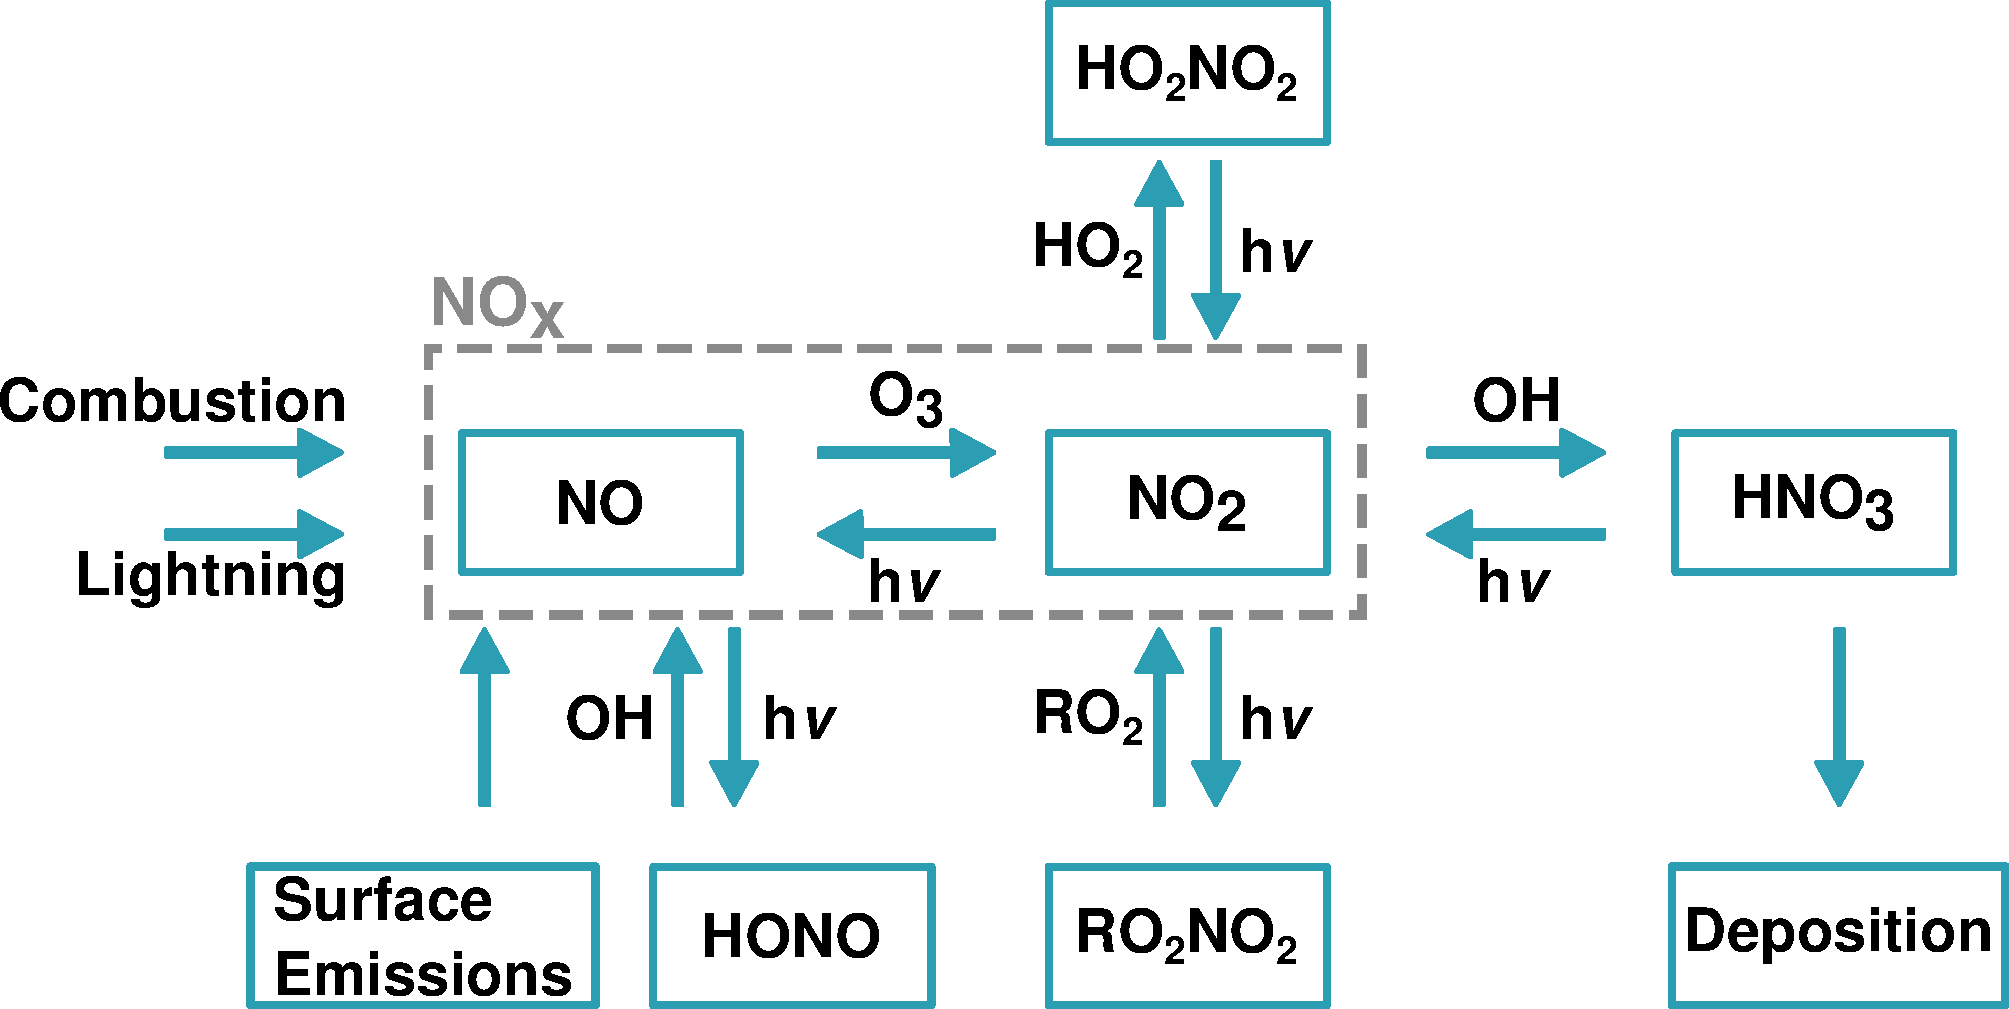
\includegraphics[width = \textwidth]{NOx_sources_sinks}%
        \label{f:NOx_sources_sinks}%
	\end{center}%
\end{figure}%

\subsection{VOCs}
This section looks at the sources of sinks of methane, non-methane VOCs and CO.
Although CO is not actually a VOC, its photochemistry is important for ozone production.
The main sink of VOCs is the oxidation chemistry (Sect.~\ref{s:ozone_chemistry}) leading to \ce{CO2} and \ce{H2O}.
The degradation of VOCs plays an important role in SOA (secondary organic aerosol) formation as well as ozone production \citep{Hallquist:2009}.

The degradation of a VOC yields the maximum possible amount of ozone when every peroxy radical converts NO to \ce{NO2} called the \emph{ozone production potential} (OPP) of a VOC.
In reality, the OPP of a VOC is never achieved as other reactions with peroxy radicals occur however the OPP is useful for assessing the amount of ozone produced from emitted VOCs.

\subsubsection{Carbon Monoxide}
Carbon monoxide is emitted directly into the troposphere through combustion and industrial processes.
An equally-important source of CO is its formation during VOC degradation.
\citet{Hauglustaine:1998} estimated that $881$~Tg~yr$^{-1}$ of CO was produced globally from chemical oxidation of VOC while $1219$~Tg~yr$^{-1}$ of CO was directly emitted.

The reaction between CO and OH \eqref{r:CO_OH} is the main sink of CO.
The OPP of CO is one as the degradation of CO produces one peroxy radical (\ce{HO2}), thus a maximum of one molecule of ozone may be produced during CO degradation.

\subsubsection{Methane}
Emissions of methane range between $500$ and $600$~Tg~\ce{CH4}~yr$^{-1}$ with $\sim$~$60$~\% of the emissions from anthropogenic sources.
The main anthropogenic sources of \ce{CH4} are agriculture, fossil fuels and biomass burning with agriculture contributing $60$~\% of the anthropogenically emitted \ce{CH4}.
Emissions from wetlands are the main natural source of methane emissions \citep{Kirschke:2013}.

Methane has a lifetime in the atmosphere of about $10$~years, significantly longer than other VOCs \citep{Voulgarakis:2013}.
The lifetime of a chemical species is the time required for the concentration of the species to decrease by $\frac{1}{e}$ \citep{Seinfeld:2006}.
Thus, methane influences ozone production on the global rather than the regional scale and is important for background levels of ozone.  

Reaction with OH \eqref{r:CH4_OH} is the main sink of methane and the secondary degradation of \ce{CH4} (Fig.~\ref{f:CH4_oxidation}) produces CO and four peroxy radicals ($1 \times$ \ce{CH3O2}, $3 \times$ \ce{HO2}).
Thus the OPP of methane is five as methane degradation can produce a maximum five molecules of \ce{O3} per molecule of \ce{CH4} oxidised. 

\subsubsection{NMVOCs}
%VOCs, types of VOCs and source (A vs B)
A wide variety of NMVOCs are emitted from anthropogenic activities directly into the troposphere.
Solvent use, industry, fossil fuel burning and transportation are all major activities emitting NMVOCs of varying functional groups, carbon numbers and reactivity.
Emissions of NMVOC from vegetation depends on meteorological variables (such as, temperature and radiation) and biological variables (such as, leaf age and leaf area index) \citep{Guenther:2012}.

\citet{Lamarque:2010} estimated that in 2000, $130$~Tg~NMVOC were globally emitted from anthropogenic sources.
This amount is dwarfed by emissions from biogenic sources -- $1000$~Tg~NMVOC~yr$^{-1}$ \citep{Guenther:2012}.
Isoprene (\ce{C5H8}) emitted from vegetation dominates at the global scale however emissions of other NMVOC from vegetation, such as monoterpenes and sesquiterpenes, may be significant on the regional scale.

Although isoprene is considered as a biogenic VOC (BVOC), it has been measured in the urban areas of London and Paris away from biogenic emission sources and during times where biogenic emissions are not important, such as freezing conditions in winter.
Transport of isoprene is unlikely as isoprene is a highly reactive NMVOC indicating anthropogenic sources of isoprene \citep{vonSchneidemesser:2011}.
Other NMVOC emitted from anthropogenic sources, such as methanol and acetaldehyde, are also emitted from vegetation \citep{Guenther:2012}.

The maximum number of molecules of \ce{O3} produced per degradation of an emitted NMVOC depends on the type and the number of carbons of the NMVOC leading to a wide range of OPPs for different NMVOC.
Unsaturated NMVOC, such as alkenes, tend to have larger OPPs than alkanes (saturated NMVOC).
Even within a functional group of NMVOC different OPPs are calculated.
For example, benzene and xylene are both aromatic compounds but as benzene is a more chemically stable molecule it has a lower OPP than xylene \citep{Carter:1994}.

OPPs for complex NMVOCs have been calculated using models by incrementally varying the concentration of an NMVOC and calculating the change in ozone.
Different OPP scales have been developed using different \ce{NO_x} conditions.
The Maximum Incremental Reactivity (MIR) and Maximum Ozone Incremental Reactivity scales of \citet{Carter:1994} and the Tagged Ozone Production Potential (TOPP) of \citet{Butler:2011} are examples of OPP scales for NMVOCs.

\subsection{Representing NMVOC Emissions in Models}
%representation of VOC emissions in models using emission inventories
Emissions of NMVOC species are a critical input in models and emission inventories are used to specify the type and quantity of emissions from source categories.
Table~\ref{t:SNAP} lists the source sectors of emissions used by the TNO-MACCIII emission inventory \citep{Kuenen:2014}.
Emission inventories are available for global or regional emissions.
For example, EDGAR \citep{Olivier:2001} specifies global emissions while TNO-MACCII \citep{Kuenen:2014} specifies European emissions.
\begin{table}[t]%
    \centering%
    \caption[Emission source sectors in the TNO\_MACCIII]{Emission source sectors for anthropogenic emissions listed in the TNO-MACCIII inventory \citep{Kuenen:2014}.}%
    \begin{tabular}{ll}%
        \hline \hline
        \textbf{Emission Source Category} & \textbf{Emission Source Category} \\
        \hline \hline
        Public Power & Road Transport: Others \\
        Residential Combustion & Road Transport: Evaporation \\
        Industry & Road Transport: Wear \\
        Fossil Fuel & Non-road Transport \\
        Solvent Use & Waste \\
        Road Transport: Gasoline & Agriculture \\
        Road Transport: Diesel & \\ 
        \hline \hline
    \end{tabular}%
    \label{t:SNAP}%
\end{table}% 

Many uncertainties are associated with emission inventories.
For example, \citet{Coll:2010} showed that large discrepancies arise between ambient measurements and emission inventories.
Often temporal variation of emissions are not captured by emission inventories \citep{Boynard:2014}. 

BVOC emissions depend on meteorological and biological variables and algorithms estimating BVOC emissions may be calculated as part of the model simulation instead of an emission inventory.
Emissions of AVOCs may also depend on meteorological variables, for example, evaporative emissions increase with temperature \citep{Rubin:2006}.
The Model of Emissions of Gases and Aerosols from Nature (MEGAN) \citep{Guenther:2006, Guenther:2012} calculates BVOC emissions using the temperature and radiation values determined from the model.
Specifiying BVOC emissions using an algorithm or emission inventory influences modelled ozone concentrations. 
For example, \citet{Curci:2009} noted large differences in summertime ozone concentrations over Europe when using a gridded emission inventory or an on-line algorithm for BVOC emissions.

%emissions in models - lumping
Emissions of the NMVOCs specified by an emission inventory are mapped to the chemical mechanism species used in the model.
This mapping is not standardised throughout the modelling community with the same NMVOC emissions possibly being allocated to different chemical species even if using the same chemical mechanism \citep{Carter:2015}.

The influence of the speciation of NMVOC emissions on modelled ozone production is determined as part of this work.
Moreover, the effect of using the same speciations of NMVOC emissions with different chemical mechanisms is also explored.
Section~\ref{s:research_questions} outlines the research questions and the results are presented in Sect.~\ref{s:EI_results}.

\section{Effects of Meteorology on Ozone Production} \label{s:meteo_ozone}
\begin{table}[t]%
    \centering%
    \caption[Influence of meteorological variables on ozone production]{Influence of meteorological variables on ozone production, taken from \citet{Jacob:2009}.}%
    \begin{tabular}{ll}%
        \hline \hline
        \textbf{Meteorological Variable} & \textbf{Influence on Ozone} \\
        \hline \hline
        Temperature & Consistently positive \\
        Stagnation & Consistently positive \\
        Wind Speed & Generally negative \\
        Mixing Height & Weak or variable \\
        Humidity & Weak or variable \\
        Cloud Cover & Generally negative \\
        Precipitation & Weak or variable \\
        \hline \hline
    \end{tabular}%
    \label{t:meteo_vars}%
\end{table}%
%metereology impacts 
Meteorological conditions influence the production of ozone with clear and calm summer days typically having high ozone levels \citep{Duenas:2002}.
\citet{Comrie:1997} noted a complex relationship between meteorology and ozone due to competing positive and negative effects on ozone production.
Table~\ref{t:meteo_vars}, taken from \citet{Jacob:2009}, details the effects of specific meteorological variables on ozone production.

Climate change is predicted to influence many meteorological variables and increase the number of heatwaves \citep{Karl:2003}.
Thus understanding the influence of meteorology on ozone production is particularly important for future predictions of air quality and tackling ozone pollution in a changing climate.

\subsubsection{Humidity}
Humidity influences ozone production both positively and negatively.
When \ce{O(^1D)}, originating from ozone photolysis \eqref{r:O3_hvb} reacts with water vapour \eqref{r:O1D_H2O}, the production of OH radicals leads to ozone loss.
However, the initiation of VOC degradation through reaction with OH can lead to ozone production (Sect.~\ref{s:ozone_chemistry}).
These competing effects of water vapour on ozone production lead to a weak correlation of ozone production with water vapour \citep{Jacob:2009}.

\subsubsection{Wind Speed}
High wind speeds transport ozone precursors away from their sources leading to a generally negative effect on ozone pollution over a region.
Model projections of \citet{Doherty:2013} showed that while climate change is expected to change large-scale atmospheric transport there is little influence on the spatial patterns of mean concentrations of ozone.

\subsubsection{Stagnation}
During periods of low wind speeds, emissions of ozone precursors remain close to their sources.
These stagnant conditions over polluted urban areas are highly correlated with increased ozone production over urban areas \citep{Jacob:2009}.
Heatwaves result from stagnant conditions along with high temperatures enhancing the ozone pollution over a region.

\subsubsection{Mixing Height}
The effects of the mixing height of the planetary boundary layer (PBL) with the free troposphere depend on the region.
For example, \citet{Dawson:2007} found that over the Eastern U.S., regions with low ozone are positively correlated with a higher mixing height whereas regions with high ozone levels are negatively affected.
This spatial effect of mixing height on ozone production depends on the difference between ozone levels within the PBL and the free troposphere \citep{Jacob:2009}.

Mixing between the PBL and free troposphere into regions with levels of surface ozone lower than the free troposphere is an additional source of ozone.
Conversely, mixing of the elevated levels of ozone from polluted areas into the free troposphere reduces the burden of surface ozone.

\subsubsection{Cloud Cover}
Cloud cover negatively affects the photochemistry of ozone production with increased cloud cover reducing the amount of sunlight reaching the troposphere.
\citet{Korsog:1991} showed a negative correlation between cloud cover and ozone and ozone levels in the study of \citet{Dawson:2007} were not significantly influenced by changes in cloud cover.

\subsubsection{Precipitation}
Precipiation influences the wet deposition rates of ozone and other chemical species.
The studies of \citet{Dawson:2007} and \citet{Murazaki:2006} noted a minor influence of precipitation on ozone levels.

\subsubsection{Temperature}
Temperature is positively correlated with ozone in many areas.
\citet{Otero:2016} showed that temperature was the main driver of summertime ozone values over many areas of central Europe while \citet{Camalier:2007} correlated ozone with temperature over the Eastern US.
\citet{Sillman:1995a} illustrated that only ozone pollution produced from the chemistry described in Sect.~\ref{s:ozone_chemistry} is correlated with temperature rather than background ozone, the ozone levels without the influence of local emissions of anthropogenic NMVOCs.

Temperature directly influences ozone levels in two ways: increasing the emissions of VOCs from vegetation and speeding up the rates of chemical reactions.
The review of \citet{Pusede:2015} showed that the temperature dependence of radical production, organic reactivity, the shorter lifetime of \ce{RO2NO2} and the formation of alkyl nitrates \eqref{r:RO2_NOb} affects ozone production.

There is a lack of detailed process studies separating the direct effects of temperature on ozone over differing \ce{NO_x} conditions despite observational and regional modelling studies correlating temperature with ozone production. 
The final part of this work addresses whether the increase in BVOC emissions or faster reaction rates with temperature is more important for ozone production.
The research questions for this study are detailed in Sect.~\ref{s:research_questions} and results are presented in Sect.~\ref{s:T-O3_results}.

\section{Research Questions and Objectives of this Thesis} \label{s:research_questions}
The detailed chemistry producing ozone cannot be fully represented in models for reasons of computational efficiency.
Thus models select a particular representation of atmospheric chemistry raising the overarching research questions for this thesis:
\begin{itemize}
    \item How do representations of detailed atmospheric chemistry influence simulated ozone production?
    \item What are the most important chemical processes when simulating ozone production?
\end{itemize}
These questions are addressed in this work through detailed modelling studies highlighting the chemical processes having the largest impact on simulated ozone production under three different conditions.

Firstly, different simplified versions of the ozone production chemistry are available to the modelling community with comparison studies showing that ozone concentrations vary between chemical mechanisms.
These chemical mechanism comparison studies do not determine the root causes of the differences between chemical mechanisms, leading to the research questions:
\begin{itemize}
	\item How do the simplification techniques used by different chemical mechanisms affect ozone production? 
    \item Which processes are responsible for differences in ozone production with different chemical mechanisms?
\end{itemize}

Secondly, NMVOC emissions are a known source of uncertainty in modelling experiments.
The choice of emission inventory influences the speciation of individual NMVOC emissions possibly influencing ozone production.
By comparing the ozone produced using different emission inventories, the following research questions are addressed:
\begin{itemize}
	\item What is the influence on modelled ozone production when using different speciations of emitted NMVOCs? 
    \item Does this influence change when using different chemical mechanisms?
\end{itemize}

Finally, meteorology influences ozone production with temperature having the strongest positive correlation with ozone.
Temperature directly influences ozone production through increasing biogenic emissions and speeding up the reaction rates of chemical reactions.
\begin{itemize}
    \item Are temperature-dependent emissions or chemical processes more important for ozone production with increasing temperature? 
    \item How is the ozone-temperature relationship treated by different chemical mechanisms?
\end{itemize}

Detailed processed studies were performed using a box model to address these research questions, details of the experimental setup are presented in Chap.~\ref{c:methodology}.
The results of the experiments are found in Chap.~\ref{c:papers}, the general discussion and conclusions of the thesis are in Chap.~\ref{c:conclusions}.
